\documentclass{article}
\usepackage{amsmath}
\usepackage{graphicx} % Required for inserting images

\title{Overview Markov Properties}
\author{Max Lang}
\date{January 2024}

\begin{document}

\section{Undirected Graphs}
\subsection{Pairwise Markov Property}
\subsubsection{Definition Pairwise Markov Property}
Let $\mathcal{G}$ be a graph with vertices $V$, and let $p$ be a probability distribution over the random variables $X_V$. We say that $p$ satisfies the pairwise Markov property for $\mathcal{G}$ if
$$
i \sim j \text { in } \mathcal{G} \Longrightarrow X_i \Perp X_j \mid X_{V \backslash\{i, j\}}[p] .
$$

In other words, whenever an edge is missing in $\mathcal{G}$ there is a corresponding conditional independence in $p$.

\subsubsection{Intuition and Example}

The \textbf{pairwise Markov property} is a fundamental concept in the context of graphical models, particularly in undirected graphical models or Markov random fields. It provides a framework for understanding the conditional independence between random variables in a probabilistic model.

Consider the undirected graph in Figure 4.2, where vertices (nodes) represent random variables $X_1, X_2, X_3,$ and $X_4$. The edges between these vertices indicate direct probabilistic interactions between the variables.

\begin{figure}[h]
    \centering
    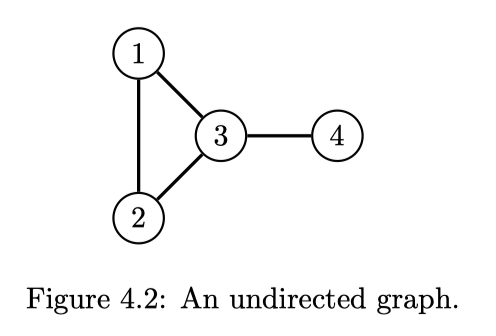
\includegraphics{overviews/graphical-models/figures/figure_4.2.png}
    \label{fig:graph}
\end{figure}

According to the pairwise Markov property:

\begin{enumerate}
    \item If there is \textit{no edge} between two vertices in the graph, the corresponding random variables are conditionally independent given all other variables. In other words, knowing the value of one does not provide any information about the other, if the values of the rest are already known.
    \item In Figure 4.2, the absence of an edge between $X_1$ and $X_4$ implies that $X_1$ and $X_4$ are conditionally independent given $X_2$ and $X_3$. Similarly, $X_2$ and $X_4$ are conditionally independent.
\end{enumerate}

Intuitively, the pairwise Markov property simplifies the understanding of complex relationships between variables. It suggests that if there is no direct "path" (edge) connecting two variables, they do not "communicate" directly, considering the influence of all other variables in the system. 

Moreover, if the distribution is positive, this property extends using Property 5 of Theorem 2.6, leading to the conclusion that $X_1, X_2$ are conditionally independent of $X_4$ given $X_3$. This stems from the fact that $X_3$ is the only variable that directly interacts with $X_4$, acting as a "gatekeeper" for information flow to $X_4$.

This concept is analogous to Markov chains, where the future state depends only on the current state, not on the sequence of events that preceded it. In a Markov network, the probability distribution over a set of variables is understood in terms of local interactions, as represented by the graph's edges.
\subsection{Global Markov Property}
\subsubsection{Definition Global Markov Property}
We say that $p$ satisfies the global Markov property for $\mathcal{G}$ if for any disjoint sets $A, B, S$
$$
A \perp_s B \mid S \text { in } \mathcal{G} \Longrightarrow X_A \Perp X_B \mid X_S[p] .
$$

In other words, whenever a separation is present in $\mathcal{G}$ there is a corresponding conditional independence in $p$.

\subsection{Intuition and Example}
\begin{itemize}
    \item \textbf{Disjoint Sets}: In a graph representing random variables, consider three sets of nodes A, B, and S, which are disjoint from each other, meaning they do not share any nodes.
    \item \textbf{Separation}: If set S separates sets A and B in the graph (i.e., S blocks all paths from any node in A to any node in B), then the random variables corresponding to A and B are conditionally independent given the random variables corresponding to S.
\end{itemize}

\begin{figure}
    \centering
    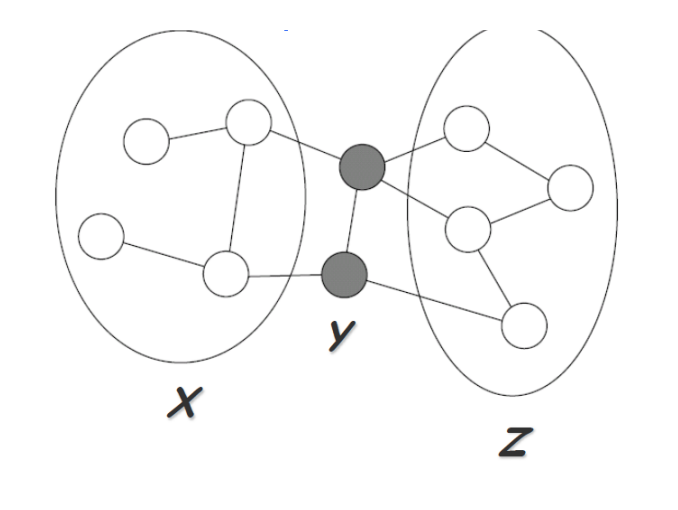
\includegraphics[width=0.5\linewidth]{overviews/graphical-models/figures/figure_GMP.png}
\end{figure}

The global Markov property generalizes the pairwise Markov property. While the pairwise property considers conditional independence between individual pairs of nodes given the rest, the global property considers conditional independence between entire sets of nodes given another set.

Intuitively, you can think of the nodes in set S as a kind of "wall" or "barrier" that blocks information flow between the nodes in sets A and B. Knowing the values of the nodes in S is sufficient to "disconnect" the probabilistic relationship between A and B.

For example, in a social network graph modeling friendships, if person S is the only mutual friend between person A and person B, then A's relationship with B can be completely explained by their relationships with S. If we know S's relationship status with both A and B, additional information about A does not change what we know about B, and vice versa, because all the information "flows" through S.



\section{Directed Graphs}
\end{document}
